\documentclass[11pt]{article}
\usepackage{color, array, graphics}
\usepackage{amsmath}
\usepackage{amssymb}
\usepackage{enumerate}
\usepackage{mathtools}
\usepackage{fullpage}
\usepackage{graphicx}
\usepackage{float}
\usepackage{listings}
\usepackage[utf8]{inputenc}

\begin{document}
\lstset{stringstyle=\ttfamily,
	showstringspaces=false,
	basicstyle=\small}

\begin{center} Alexander Garcia \hfill June 19, 2017 \\ Assignment-4 \end{center}

\medskip

\begin{enumerate}

	\item Data: $[(0,0),(1,1),(2,3)]$

		\begin{enumerate}[(a)]

			\item A full degree polynomial interpolation using the Lagrange basis is by definition

			\[
				y = \sum_{i = 1}^{n} y_i L_i(x_i)
			\]
			where
			\[
				L_i = \prod_{k = 1\ k \neq i}^{n} \frac{x-x_k}{x_i-x_k}
			\] \

			In this case, $n=3$ and

			\begin{tabular}{lll}
				$x_1 = 0$ & $x_2 = 1$ & $x_3 = 2$ \\
				$y_1 = 0$ & $y_2 = 1$ & $y_3 = 3$ \\
			\end{tabular} \\

			$y = 0L_1(x_1) + 1L_2(x_2) + 3L_3(x_3)$

			\[
				L_2 = \frac{x-0}{1-0} * \frac{x-2}{1-2}
				= -x^2 + 2x
			\]

			\[
				L_3 = \frac{x-0}{2-0} * \frac{x-1}{2-1}
				= \frac{x^2-x}{2}
			\]

			\[
				y = -x^2 + 2x + \frac{3}{2}(x^2-x) = \frac{1}{2}(x^2 + x)
			\]

			Just to ensure the interpolant agrees with the data, a small MATLAB script was used to plot $y$ with the points
			overlaid.

			\begin{center}
				\texttt{holmes5\_1.m} script
			\end{center}
			\lstinputlisting{holmes5_1.m} \

			\begin{figure}[H]
				\centering
				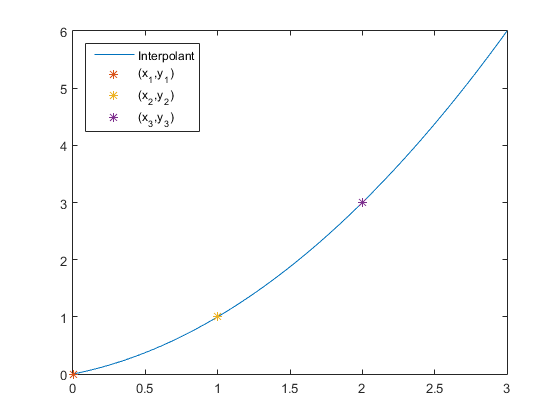
\includegraphics[width=0.5\textwidth]{holmes5_1.png}
				\caption{Graph of $y$ and the data points}
			\end{figure} \

			\item Piecewise linear interpolation for this data set consists of 2 equations $S_1(x), S_2(x)$ which
				interpolate the data between $[x_1, x_2]$, $[x_2, x_3]$ respectively.

				In general, $$S_i(x) = a_ix+b_i$$ where $$S_i(x_i) = y_i$$ From here, we get
				$$a_i = \frac{y_{i+1}-y_i}{x_{i+1}-x_i}\ \ \ \ \ b_i = y_i - \frac{y_{i+1}-y_i}{x_{i+1}-x_i}*x_i$$

				Then,
				\[
					S_1(x) = \frac{1-0}{1-0}x + (0-\frac{1-0}{1-0}*0)
					=x\ \ \ \ \ x\in[0,1]
				\]

				and
				\[
					S_2(x) = \frac{3-1}{2-1}x + (1-\frac{3-1}{2-1}*1)
					=2x - 1\ \ \ \ \ x\in[1,2]
				\]

				A simple script \texttt{holmes5\_1\_lin.m} was used to check the results of the interpolation.

				\begin{center}
					\texttt{holmes5\_1\_lin.m}
				\end{center}
				\lstinputlisting{holmes5_1_lin.m}

				\begin{figure}[H]
					\centering
					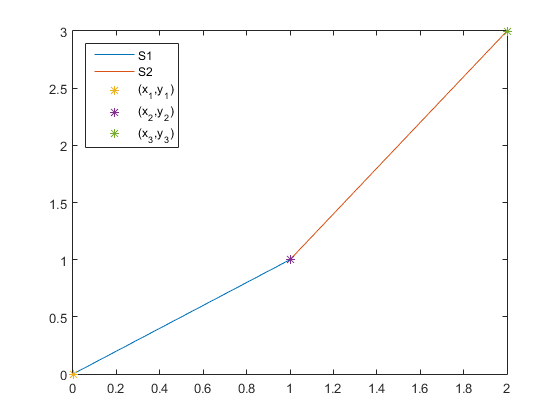
\includegraphics[width=0.5\textwidth]{holmes5_1_lin.png}
					\caption{Graph of linear piecewise interpolant}
				\end{figure} \

			\item Natural cubic spline interpolation insists that the second derivative at both the first and last data points
				are zero.

				Again, there are 2 equations $S_1(x), S_2(x)$ that interpolate the data between $[x_1, x_2]$, $[x_2,x_3]$
				respectively. In general, $$S_i(x) = a_ix^3 + b_ix^2+c_ix+d_i$$
				In order to satisfy the interpolation conditions, it must be enforced that $S_i(x_i) = y_i$. In addition, to
				ensure a smooth curve through the data, we insist that $S_i(x_i) = S_{i+1}(x_i),\ S'_i(x_i) = S'_{i+1}(x_i),\
				S''_i(x_i) = S''_{i+1}(x_i)$

				Given the initial conditions, we can construct a matrix to solve for the coefficients $a_i, b_i, c_i, d_i$.
				Each entry in matrix $\mathbf{A}$ is the value of $x_i$ raised to the corresponding power.

				\[
					\begin{bmatrix}
						0 & 0 & 0 & 1 & 0 & 0 & 0 & 0\\
						1 & 1 & 1 & 1 & 0 & 0 & 0 & 0\\
						0 & 0 & 0 & 0 & 1 & 1 & 1 & 1\\
						0 & 0 & 0 & 0 & 8 & 4 & 2 & 1\\
						6 & 2 & 0 & 0 &-6 &-2 & 0 & 0\\
						3 & 2 & 1 & 0 &-3 &-2 &-1 & 0\\
						0 & 2 & 0 & 0 & 0 & 0 & 0 & 0\\
						0 & 0 & 0 & 0 &12 & 4 & 0 & 0\\
					\end{bmatrix}
					\begin{bmatrix}
						a_1 \\
						b_1 \\
						c_1 \\
						d_1 \\
						a_2 \\
						b_2 \\
						c_2 \\
						d_2 \\
					\end{bmatrix}
					=
					\begin{bmatrix}
						0 \\
						1 \\
						1 \\
						3 \\
						0 \\
						0 \\
						0 \\
						0 \\
					\end{bmatrix}
				\] \\

				A brief explanation of the contents of this matrix:

				\begin{tabular}{cl}
					Rows 1-4: & Interpolation conditions; $S_i(x_i) = y_i$ \\
					Rows 5-6: & ``Smoothness'' conditions; agreeing first and second derivatives \\
					Rows 7-8: & Natural spline conditions; zero end point second derivatives \\
				\end{tabular} \

				Solving this system using the backslash command in MATLAB yields

				\[
					\mathbf{c}=
					\begin{bmatrix}
						0 & 0 & 1 & 0 & 1 & -3 & 4 & -1 \\
					\end{bmatrix}^T
				\]

				Using these results, we have $$S_1(x) = x$$ and $$S_2(x) = x^3 - 3x^2 + 4x - 1$$
				Below is the script used to both calculate and plot the resulting splines.

				\begin{center}
					\texttt{holmes5\_1\_cubic.m}
				\end{center}
				\lstinputlisting{holmes5_1_cubic.m} \

				\begin{figure}[H]
					\centering
					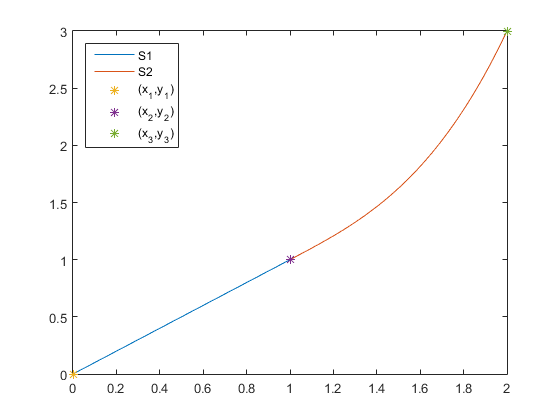
\includegraphics[width=0.5\textwidth]{holmes5_1_cubic.png}
					\caption{Graph of cubic piecewise interpolant}
				\end{figure} \

		\end{enumerate}

	\item Function to interpolate: $f(x) = sinx$

		\begin{enumerate}[(a)]

			\item Piecewise linear interpolation

				The linear spline passing through $\frac{\pi}{8}$ would be $S_1(x)$.
				$$S_1(x) = \frac{y_2-y_1}{x_2-x_1}x + (y_1 - \frac{y_2-y_1}{x_2-x_1})x_1\ \ \ \ x\in[0,\frac{\pi}{4}]$$
				$$S_1(x) = \frac{\sqrt{2}/2-0}{\pi/4-0}x + (\sqrt{2}/2 - \frac{\sqrt{2}/2-0}{\pi/4-0})0$$
				$$= \frac{\sqrt{2}/2}{\pi/4}x$$

				A MATLAB script \texttt{holmes5\_5a.m} was used to calculate the estimated value of $f(\pi/8)$, and plot
				the interpolant and the original function.

				$$S_1(\pi/8) = 0.35355$$
				$$|S_1(\pi/8) - sin(\pi/8)| = 0.02913$$ \\

				\begin{center}
					\texttt{holmes5\_5a.m}
				\end{center}
				\lstinputlisting{holmes5_5a.m} \

				\begin{figure}[H]
					\centering
					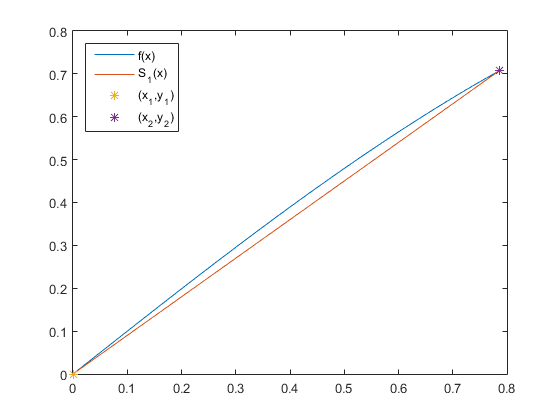
\includegraphics[width=0.5\textwidth]{holmes5_5a.png}
					\caption{Graph of $f(x)$ and $S_1(x)$}
				\end{figure} \

			\item Full degree interpolation using the Lagrange basis

				The Lagrange interpolant in this case uses $n = 3$, with data points

				\begin{tabular}{lll}
					$x_1 = 0$ & $x_2 = \frac{\pi}{4}$ & $x_3 = \frac{\pi}{2}$ \\
					$y_1 = 0$ & $y_2 = \frac{\sqrt{2}}{2}$ & $y_3 = 1$ \\
				\end{tabular}

				$y = 0L_1(x_1) + (\sqrt{2}/2)L_2(x_2) + 1L_3(x_3)$

				\[
					L_2(x_2) = \frac{x-0}{\pi/4-0}*\frac{x-\pi/2}{\pi/4-\pi/2}
					= -\frac{16x^2-8\pi x}{\pi^2}
				\]

				\[
					L_3(x_3) = \frac{x-0}{\pi/2-0} * \frac{x-\pi/4}{\pi/2-\pi/4}
					= \frac{8x^2-2\pi x}{\pi^2}
				\]

				\[
					y = -\frac{\sqrt{2}}{2}*\frac{16x^2-8\pi x}{\pi^2} + \frac{8x^2-2\pi x}{\pi^2}
					= \frac{(8-8\sqrt{2})x^2+(4\sqrt{2}\pi-2\pi)x}{\pi^2}
				\]

				Again, MATLAB was used to verify the result, as well as calculate the error.

				$$y(\pi/8) = 0.40533$$
				$$|y(\pi/8)-sin(\pi/8)| = 0.02265$$ \\

				\begin{center}
					\texttt{holmes5\_5b.m}
				\end{center}
				\lstinputlisting{holmes5_5b.m} \

				\begin{figure}[H]
					\centering
					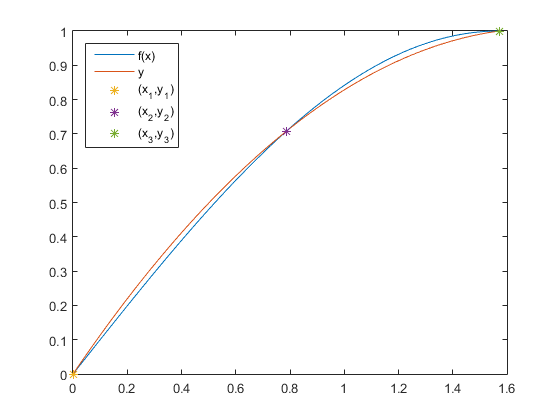
\includegraphics[width=0.5\textwidth]{holmes5_5b.png}
					\caption{Graph of $f(x)$ and full degree interpolating polynomial $y$}
				\end{figure} \

			\item Natural cubic spline interpolation \\

				\begin{tabular}{cl}
					Rows 1-4: & Interpolation conditions; $S_i(x_i) = y_i$ \\
					Rows 5-6: & ``Smoothness'' conditions; agreeing first and second derivatives \\
					Rows 7-8: & Natural spline conditions; zero end point second derivatives \\
				\end{tabular} \\

				\[
					\begin{bmatrix}
						0 & 0 & 0 & 1 & 0 & 0 & 0 & 0\\
						\pi^3/64 & \pi^2/16 & \pi/4 & 1 & 0 & 0 & 0 & 0\\
						0 & 0 & 0 & 0 & \pi^3/64 & \pi^2/16 & \pi/4 & 1\\
						0 & 0 & 0 & 0 & \pi^3/8 & \pi^2/4 & \pi/2 & 1\\
						3\pi^2/16 & \pi/2 & 1 & 0 & -3\pi^2/16 & -\pi/2 & -1 & 0\\
						3\pi/2 & 2 & 0 & 0 & -3\pi/2 & -2 & 0 & 0\\
						0 & 2 & 0 & 0 & 0 & 0 & 0 & 0\\
						0 & 0 & 0 & 0 & 3\pi & 2 & 0 & 0\\
					\end{bmatrix}
					\begin{bmatrix}
						a_1\\
						b_1\\
						c_1\\
						d_1\\
						a_2\\
						b_2\\
						c_2\\
						d_2\\
					\end{bmatrix}
					=
					\begin{bmatrix}
						0\\
						\sqrt{2}/2\\
						\sqrt{2}/2\\
						1\\
						0\\
						0\\
						0\\
						0\\
					\end{bmatrix}
				\] \\

				A MATLAB script was used to calculate the resulting coefficients, the error of the interpolating spline,
				as well as plot the spline and $f(x)$. The resulting splines are \\

				\begin{center}
				\begin{tabular}{lr}
					$S_1(x) = -0.21374x^3 + 1.03216x$ & $x\in[0,\pi/4]$ \\
					$S_2(x) = 0.21374x^3 - 1.00725x^2 + 1.82325x - 0.20711$ & $x\in[\pi/4,\pi/2]$ \\
				\end{tabular}
				\end{center}

				$$S_1(\pi/8) = 0.39239$$
				$$|S_1(\pi/8) - sin(\pi/8)| = 0.00970$$ \\

				\begin{center}
					\texttt{holmes5\_5c.m} script
				\end{center}
				\lstinputlisting{holmes5_5c.m} \

				\begin{figure}[H]
					\centering
					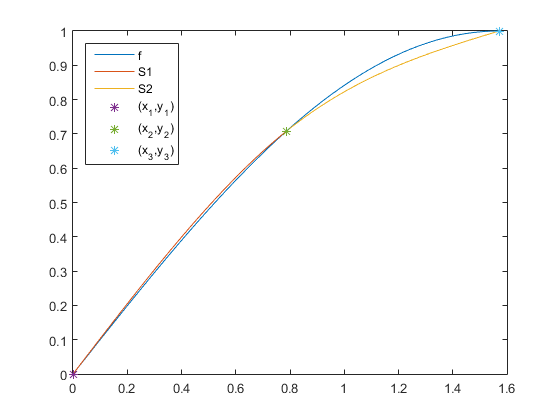
\includegraphics[width=0.5\textwidth]{holmes5_5c.png}
					\caption{Graph of $f(x)$ and natural cubic splines $S_1(x), S_2(x)$}
				\end{figure} \

			\item Clamped cubic spline interpolation \\

				\begin{tabular}{cl}
					Rows 1-4: & Interpolation conditions; $S_i(x_i) = y_i$ \\
					Rows 5-6: & ``Smoothness'' conditions; agreeing first and second derivatives \\
					Rows 7-8: & Clamped spline conditions; fixed end point first derivatives \\
				\end{tabular} \\

				\[
					\begin{bmatrix}
						0 & 0 & 0 & 1 & 0 & 0 & 0 & 0\\
						\pi^3/64 & \pi^2/16 & \pi/4 & 1 & 0 & 0 & 0 & 0\\
						0 & 0 & 0 & 0 & \pi^3/64 & \pi^2/16 & \pi/4 & 1\\
						0 & 0 & 0 & 0 & \pi^3/8 & \pi^2/4 & \pi/2 & 1\\
						3\pi^2/16 & \pi/2 & 1 & 0 & -3\pi^2/16 & -\pi/2 & -1 & 0\\
						3\pi/2 & 2 & 0 & 0 & -3\pi/2 & -2 & 0 & 0\\
						0 & 0 & 1 & 0 & 0 & 0 & 0 & 0\\
						0 & 0 & 0 & 0 & 3\pi^2/4 & \pi & 1 & 0\\
					\end{bmatrix}
					\begin{bmatrix}
						a_1\\
						b_1\\
						c_1\\
						d_1\\
						a_2\\
						b_2\\
						c_2\\
						d_2\\
					\end{bmatrix}
					=
					\begin{bmatrix}
						0\\
						\sqrt{2}/2\\
						\sqrt{2}/2\\
						1\\
						0\\
						0\\
						1\\
						0\\
					\end{bmatrix}
				\] \\

				Once again, the coefficients were calculated by a MATLAB script, as well as the error, and a plot of the
				spline and function. \\

				\begin{center}
				\begin{tabular}{lr}
					$S_1(x) = -0.34178x^3 + 0.14151x^2 + x$ & $x\in[0,\pi/4]$ \\
					$S_2(x) = 0.49355x^3 - 1.82668x^2 + 2.54582x - 0.40469$ & $x\in[\pi/4,\pi/2]$ \\
				\end{tabular}
				\end{center}

				$$S_1(\pi/8) = 0.39382$$
				$$|S_1(\pi/8) - sin(\pi/8)| = 0.01114$$ \\

				\begin{center}
					\texttt{holmes5\_5d.m} script
				\end{center}
				\lstinputlisting{holmes5_5d.m} \

				\begin{figure}[H]
					\centering
					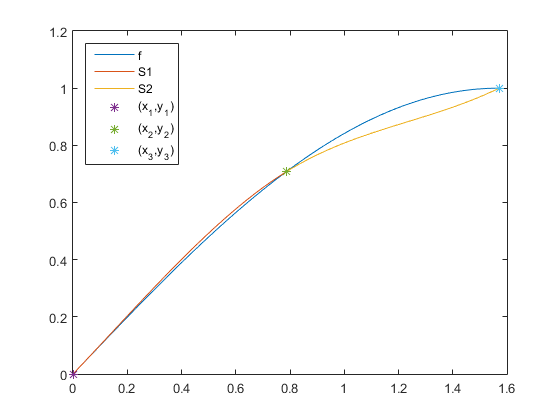
\includegraphics[width=0.5\textwidth]{holmes5_5d.png}
					\caption{Graph of $f(x)$ and clamped cubic splines $S_1(x), S_2(x)$}
				\end{figure} \

			\item Chebyshev interpolation \\

				The function needed to determine the nodes for full-degree interpolation are given by the zeros of the
				Chebyshev polynomial $T_n(x) = cosn\theta$, which occur at $n\theta = \frac{(2k-1)\pi}{2n}$, where $k=1:n$.
				However, this only applies to the interval $[-1,1]$, and therefore must be expanded to our interval $[0,
				\pi/2]$. When generalized, the zeros lie at $\frac{b+a}{2} - \frac{b-a}{2}cos(\frac{(2k-1)\pi}{2n})$, again
				with $k=1:n$. In our case then, $n = 3$, $b = \pi/2$, $a=0$, and the zeros are

				\begin{center}
				\begin{tabular}{ll}
					$k=1$: & $x_1 = \frac{\pi}{4} - \frac{\pi}{4}cos(\frac{\pi}{6}) = 0.1052$ \\
					$k=2$: & $x_2 = \frac{\pi}{4} - \frac{\pi}{4}cos(\frac{\pi}{2}) = \frac{\pi}{4}$ \\
					$k=3$: & $x_3 = \frac{\pi}{4} - \frac{\pi}{4}cos(\frac{5\pi}{6}) = 1.4656$ \\
				\end{tabular}
				\end{center}

				We then use these nodes, to generate a full degree polynomial
				interpolant, in this case using the Lagrange basis.

				$$y = y_1L_1(x_1) + y_2L_2(x_2) + y_3L_3(x_3)$$

				$$L_1(x_1) = \frac{x-\pi/4}{0.1052-\pi/4}*\frac{x-1.4656}{0.1052-1.4656}$$
				$$L_2(x_2) = \frac{x-0.1052}{\pi/4-0.1052}*\frac{x-1.4656}{\pi/4-1.4656}$$
				$$L_3(x_3) = \frac{x-0.1052}{1.4656-0.1052}*\frac{x-\pi/4}{1.4656-\pi/4}$$

				$$y(x) = sin(x_1)L_1(x_1) + sin(x_2)L_2(x_2) + sin(x_3)L_3(x_3)$$

				The function estimate, as well as the error, were calculated through a MATLAB script. The script also plots
				the interpolant and the original function. \\

				$$y(\pi/8) = 0.39790$$
				$$|y(\pi/8)-sin(\pi/8)| = 0.01521$$ \\

				\begin{center}
					\texttt{holmes5\_5e.m} script
				\end{center}
				\lstinputlisting{holmes5_5e.m} \

				\begin{figure}[H]
					\centering
					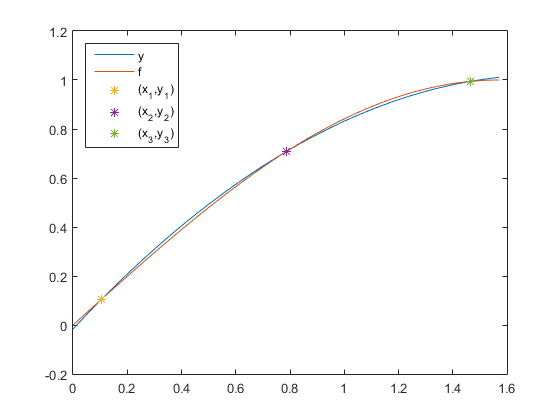
\includegraphics[width=0.5\textwidth]{holmes5_5e.png}
					\caption{Graph of $f(x)$ and the Chebyshev polynomial $y(x)$}
				\end{figure} \

		\end{enumerate}

	\item

\end{enumerate}

\end{document}
